% mnras_template.tex
%
% LaTeX template for creating an MNRAS paper
%
% v3.0 released 14 May 2015
% (version numbers match those of mnras.cls)
%
% Copyright (C) Royal Astronomical Society 2015
% Authors:
% Keith T. Smith (Royal Astronomical Society)

% Change log
%
% v3.0 May 2015
%    Renamed to match the new package name
%    Version number matches mnras.cls
%    A few minor tweaks to wording
% v1.0 September 2013
%    Beta testing only - never publicly released
%    First version: a simple (ish) template for creating an MNRAS paper

%%%%%%%%%%%%%%%%%%%%%%%%%%%%%%%%%%%%%%%%%%%%%%%%%%
% Basic setup. Most papers should leave these options alone.
\documentclass[fleqn,usenatbib]{mnras}
%\pdfminorversion=5

% MNRAS is set in Times font. If you don't have this installed (most LaTeX
% installations will be fine) or prefer the old Computer Modern fonts, comment
% out the following line
%\usepackage{newtxtext,newtxmath}
% Depending on your LaTeX fonts installation, you might get better results with one of these:
%\usepackage{mathptmx}
%\usepackage{txfonts}

% Use vector fonts, so it zooms properly in on-screen viewing software
% Don't change these lines unless you know what you are doing
\usepackage[T1]{fontenc}
\usepackage{ae,aecompl}
\usepackage{hyperref}

%%%%% AUTHORS - PLACE YOUR OWN PACKAGES HERE %%%%%

% Only include extra packages if you really need them. Common packages are:
\usepackage{graphicx}	% Including figure files
\usepackage{amsmath}	% Advanced maths commands
\usepackage{amssymb}	% Extra maths symbols
\usepackage{multirow}
\usepackage[usenames,dvipsnames,svgnames,table]{xcolor}
\usepackage{verbatim}

%\hypersetup{draft}

%%%%%%%%%%%%%%%%%%%%%%%%%%%%%%%%%%%%%%%%%%%%%%%%%%

%%%%% AUTHORS - PLACE YOUR OWN COMMANDS HERE %%%%%

% Please keep new commands to a minimum, and use \newcommand not \def to avoid
% overwriting existing commands. Example:
%\newcommand{\pcm}{\,cm$^{-2}$}	% per cm-squared

\newcommand{\homsun}{\,h^{-1} {\rm M_\odot}}
\newcommand{\hmsun}{\,h^{-2} {\rm M_\odot}}
\newcommand{\msun}{{\rm M_\odot}}
\newcommand{\hkpc}{\, h^{-1}{\rm{kpc}} }
\newcommand{\hMpc}{\, h^{-1}{\rm{Mpc}} }
\newcommand{\magn}{\, {\rm mag} }

\newcommand{\hsmsun}{\,h_{70}^{-2} {\rm M_\odot}}
\newcommand{\hskpc}{\, h_{70}^{-1}{\rm{kpc}} }
\newcommand{\hsMpc}{\, h_{70}^{-1}{\rm{Mpc}} }
\newcommand{\hsGpc}{\, h_{70}^{-1}{\rm{Gpc}} }

\newcommand{\lan}{\langle}
\newcommand{\ra}{\rangle}

\newcommand{\lcdm}{{\rm \Lambda CDM}}
\newcommand{\am}{\, {\rm arcmin}}
\newcommand{\as}{\, {\rm arcsec}}
\newcommand*{\mean}[1]{\overline{#1}}
\newcommand*{\E}[1]{\times 10^{#1}}

\newcommand*{\swap}[2]{#2#1}

%%%%%%%%%%%%%%%%%%%%%%%%%%%%%%%%%%%%%%%%%%%%%%%%%%

%%%%%%%%%%%%%%%%%%% TITLE PAGE %%%%%%%%%%%%%%%%%%%

% Title of the paper, and the short title which is used in the headers.
% Keep the title short and informative.
\title[Trough and Ridge Lensing with KiDS]{Studying galaxy troughs and ridges using Weak Gravitational Lensing with the Kilo-Degree Survey}
% The list of authors, and the short list which is used in the headers.
% If you need two or more lines of authors, add an extra line using \newauthor
\author[M. M. Brouwer et al.]{Margot M. Brouwer$^{1,2}$\thanks{E-mail:brouwer@astro.rug.nl},
	 %Group 1:
	 %Group 2:
	 %Group 3:
	\\
	\\
	% List of institutions
	$^{1}$Kapteyn Astronomical Institute, University of Groningen, PO Box 800, NL-9700 AV Groningen, the Netherlands.\\
	$^{2}$Institute for Theoretical Physics, University of Amsterdam, Science Park 904, 1098 XH Amsterdam, The Netherlands. \\
}

% These dates will be filled out by the publisher
\date{Accepted XXX. Received YYY; in original form ZZZ}

% Enter the current year, for the copyright statements etc.
\pubyear{2019}

% Don't change these lines
\begin{document}
\label{firstpage}
\pagerange{\pageref{firstpage}--\pageref{lastpage}}
\maketitle

% Abstract of the paper
\begin{abstract}
TBW
\end{abstract}


% Select between one and six entries from the list of approved keywords.
% Don't make up new ones.
\begin{keywords}
gravitational lensing: weak -- Surveys -- methods: statistical -- galaxies: haloes -- cosmology: dark matter, theory -- gravitation.
\\
\end{keywords}

%\newpage
\clearpage

%%%%%%%%%%%%%%%%%%%%%%%%%%%%%%%%%%%%%%%%%%%%%%%%%%

%%%%%%%%%%%%%%%%% BODY OF PAPER %%%%%%%%%%%%%%%%%%


\section{Introduction}
\label{sec:introduction}
Write the beginning

\section{Data}
\label{sec:data}

\subsection{KiDS source galaxies}
\label{sec:kids}
Write the beginning.
Need to know:
\begin{itemize}
	\item What changes as we go to KiDS-1000 (K1000 paper?).
\end{itemize}

\subsection{GAMA foreground galaxies}
\label{sec:gama}
Write the whole.

\subsection{KiDS foreground selection}
\label{sec:gamalike_kids}
Still need to know:
\begin{itemize}
	\item Maciek's GL-KiDS selection criteria for K1000.
	\item Angus' stellar mass method for K1000.
\end{itemize}

\subsection{MICE mock galaxies}
\label{sec:mice_mocks}
Write the whole.

\subsection{Bahamas mock galaxies}
\label{sec:bahamas_mocks}
Written by Kyle?

\section{Data analysis}
\label{sec:analysis}

\subsection{Isolated galaxy selection}
\label{sec:isolation}
Write the beginning.
Still need to know:
\begin{itemize}
	\item how to test the isolation criterion.
\end{itemize}

\subsection{Lensing measurement}
\label{sec:lensing}
Write the beginning.
Still need to know:
\begin{itemize}
	\item How (if?) the GGL-pipeline changes with K1000.
\end{itemize}

\begin{comment}
In order to measure the projected mass density of the selected troughs and ridges, we use weak gravitational lensing \cite[see][for a general introduction]{bartelmann2001,schneider2006}. This method measures systematic tidal distortions of the light from many background galaxies (sources) by foreground mass distributions (lenses). This gravitational deflection causes a distortion in the observed shapes of the source images of $\sim 1\%$, which can only be measured statistically. This is done by averaging, from many background sources, the projected ellipticity component $\epsilon_{\rm t}$ tangential to the direction towards the centre of the lens, which is an estimator of the `tangential shear' $\gamma_{\rm t}$. This quantity is averaged within circular annuli around the center of the lens, to create a shear profile $\gamma_{\rm t}(\theta)$ as a function of the separation angle $\theta$ to the lens centre. For each annulus, $\gamma_{\rm t}(\theta)$ is a measure of the density contrast of the foreground mass distribution. In order to obtain a reasonable signal-to-noise ratio ($S/N$), the shear measurement around many lenses is `stacked' to create the average shear profile of a specified lens sample. In this work, the centres of the lenses are the grid points that define our circular troughs and ridges (as defined in Sect. \ref{sec:trough_selection}).

The background sources used to measure the lensing effect are the KiDS galaxies described in Sect. \ref{sec:kids}. Following \cite{hildebrandt2017}, we only use sources with a best-fit photometric redshift $0.1<z_{\rm B}<0.9$. For troughs defined at a specific redshift we only select sources situated beyond the troughs, including a redshift buffer of $\Delta z=0.2$ (see Sect. \ref{sec:esd_measurements}). This cut is not applied when troughs are selected over the full redshift range. This can allow sources that reside at similar redshifts as the lenses to be used in the measurement, which would result in a contamination of the lensing signal by sources that are not lensed (`boost factor') and/or by sources that are intrinsically aligned with the troughs. However, even without a redshift cut $80\%$ of the KiDS source galaxies have a best-fit photometric redshift $z_{\rm B}$ above the mean redshift ($\mean{z_{\rm G}} = 0.24$) of our GAMA sample. Also, the intrinsic alignment effect has proven to be very small and difficult to detect, and primarily plays a role in very high-density regions on small ($\lesssim 1 \hsMpc$) scales. On the large scales probed by the troughs, the contamination of the lensing signal from intrinsic alignment is expected to be at most a few percent \cite[]{heymans2006,blazek2012}. Regarding the boost factor, this effect is also reproduced in the results obtained from the mock catalogues to which we compare our observations.

The ellipticities of the source galaxies are measured using the self-calibrating \emph{lens}fit pipeline \cite[]{miller2007,miller2013,fenechconti2017}. For each galaxy this model fitting method also produces the \emph{lens}fit weight $w$, which is a measure of the precision of the shear estimate it provides. We incorporate the \emph{lens}fit weight of each source into the average tangential shear in each angular bin as follows:
\begin{equation}
\mean{\gamma} = \frac{1}{1+\mu} \frac{\sum_{ls} w_{s} \, \epsilon_{{\rm t},ls} }{ \sum_{ls}{w_{s}} }  \, .
\label{eq:shear_measured}
\end{equation}
Here the sum goes over each lens $l$ in the lens sample (e.g. all apertures with a specified size and galaxy number density) and over each source $s$ inside the considered bin in angular separation from the centre of the lens. The factor $1+\mu$ is used to correct for `multiplicative bias'. Based on extensive image simulations \cite{fenechconti2017} showed that, on average, shears are biased at the $1-2\%$ level, and how this can be corrected using a multiplicative bias correction $m$ for every ellipticity measurement. Following \cite{dvornik2017}, the value of $\mu$ is calculated from the $m$-corrections in $8$ redshift bins (with a width of $0.1$) between $0.1 < z_{\rm B} < 0.9$. The average correction in each bin is defined as follows:
\begin{equation}
\mu=\frac{\sum_{s} w_{s} m_{s}}{\sum_{ls} w_{s}} \, .
\label{eq:biascorr}
\end{equation}
The required correction is small ($\mu\approx0.014$) independent of angular separation, and reduces the residual multiplicative bias to $\lesssim1\%$. The errors on our shear measurement are estimated by the square-root of the diagonal of the analytical covariance matrix (see Sect. \ref{sec:covariance}). The analytical covariance is based on the contribution of each individual source to the lensing signal, and takes into account the covariance between sources that contribute to the shear profile of multiple lenses. Its calculation is described in Sect. 3.4 of \cite{viola2015}.

In addition to measuring the lensing profile around troughs and ridges, we stack the shear around \emph{all} grid points ($262\,507$ in the case of KiDS, $112\,500$ in the case of GAMA). In accordance with the real trough measurements, the apertures with an effective area less than $80\%$ of the total circle area are removed (see Sect. \ref{sec:trough_selection}). This `random' tangential shear signal, that we henceforth denote as $\gamma_0$, does not contain a coherent shear profile, but only systematic effects resulting from the imperfect correction of any low-level PSF anisotropy in combination with the survey edges and masks. Subtracting $\gamma_0$ from our shear profiles will both remove these systematic effects and reduce the noise in the measured signals \cite[]{gruen2017,singh2017}. The random signals for KiDS and GAMA are shown in Fig. \ref{fig:kids_vs_gama_randoms}. When using the GAMA survey area and mask, $\gamma_0$ is consistent with zero (within $1\sigma$ error bars) up to $\theta = 70 \am$, where it rises to $\gamma_0 \sim 3\E{-3}$ for all values of $\theta_{\rm A}$, while the KiDS random signal already starts to deviate from zero at $\theta \approx 20 \am$. This difference does not significantly depend on the choice of area completeness threshold, and also occurs when we apply no completeness mask at all. However, when we perform the $\gamma_0$ measurement using the KiDS mask on the GAMA area only, the systematic effect is significantly reduced. This shows that the difference between the random signals is primarily caused by the patchy surface coverage of the KiDS-450 dataset beyond the GAMA area \cite[see e.g. Fig. 1 of][]{hildebrandt2017}. The same effect can be seen in Fig. 15 of \cite{uitert2016b}, who conclude that it originates from the boundaries of the survey tiles.

To correct for this effect at larger scales, we subtract the appropriate $\gamma_0$ from all lensing measurements in this work. Based on the radius where the random signal becomes significant ($\theta\sim70 \am$), and on our grid spacing of $0.04 \deg = 2.4 \am$ (see Sect. \ref{sec:trough_selection}), we compute our lensing profiles within the angular separation: $2 < \theta < 100 \am$. We split this range into 20 logarithmically spaced bins.
\end{comment}

\subsection{Conversion to radial acceleration}
\label{sec:conversion}
Still need to know: whether we will use the SIS assumption or linear interpolation.
\begin{itemize}
	\item Test the SIS assumption using the Bahamas simulation.
\end{itemize}
	
\subsection{Theoretical predictions}
\label{sec:predictions}

\subsubsection{Analytical CDM model}
\label{sec:analytical}
Written by Kyle?

\subsubsection{Modified Newtonian Gravity}
\label{sec:MOND}
Write the whole.

\subsubsection{Emergent Gravity}
\label{sec:EG}
Write the whole.

\section{Results}
\label{sec:results}
Write when the results are ready.
I still need:
\begin{itemize}
	\item The K1000 lensing catalogues with ANNz redshifts and stellar masses.
	\item The results from the Bahamas simulation.
\end{itemize}

\subsection{Isolated galaxies}

\begin{figure}
	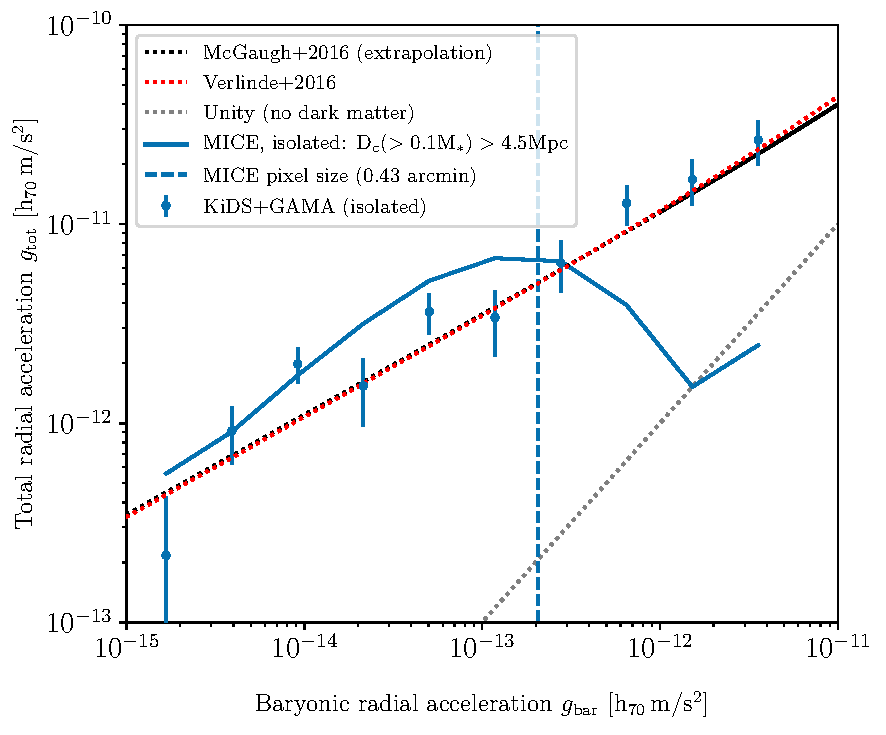
\includegraphics[width=1.0\columnwidth]{Figures/RAR_GAMA+MICE_isolated_strong.pdf}
	\caption{TBW}
	%\label{fig:}
\end{figure}

\subsection{Stellar mass bins}

\begin{figure*}
	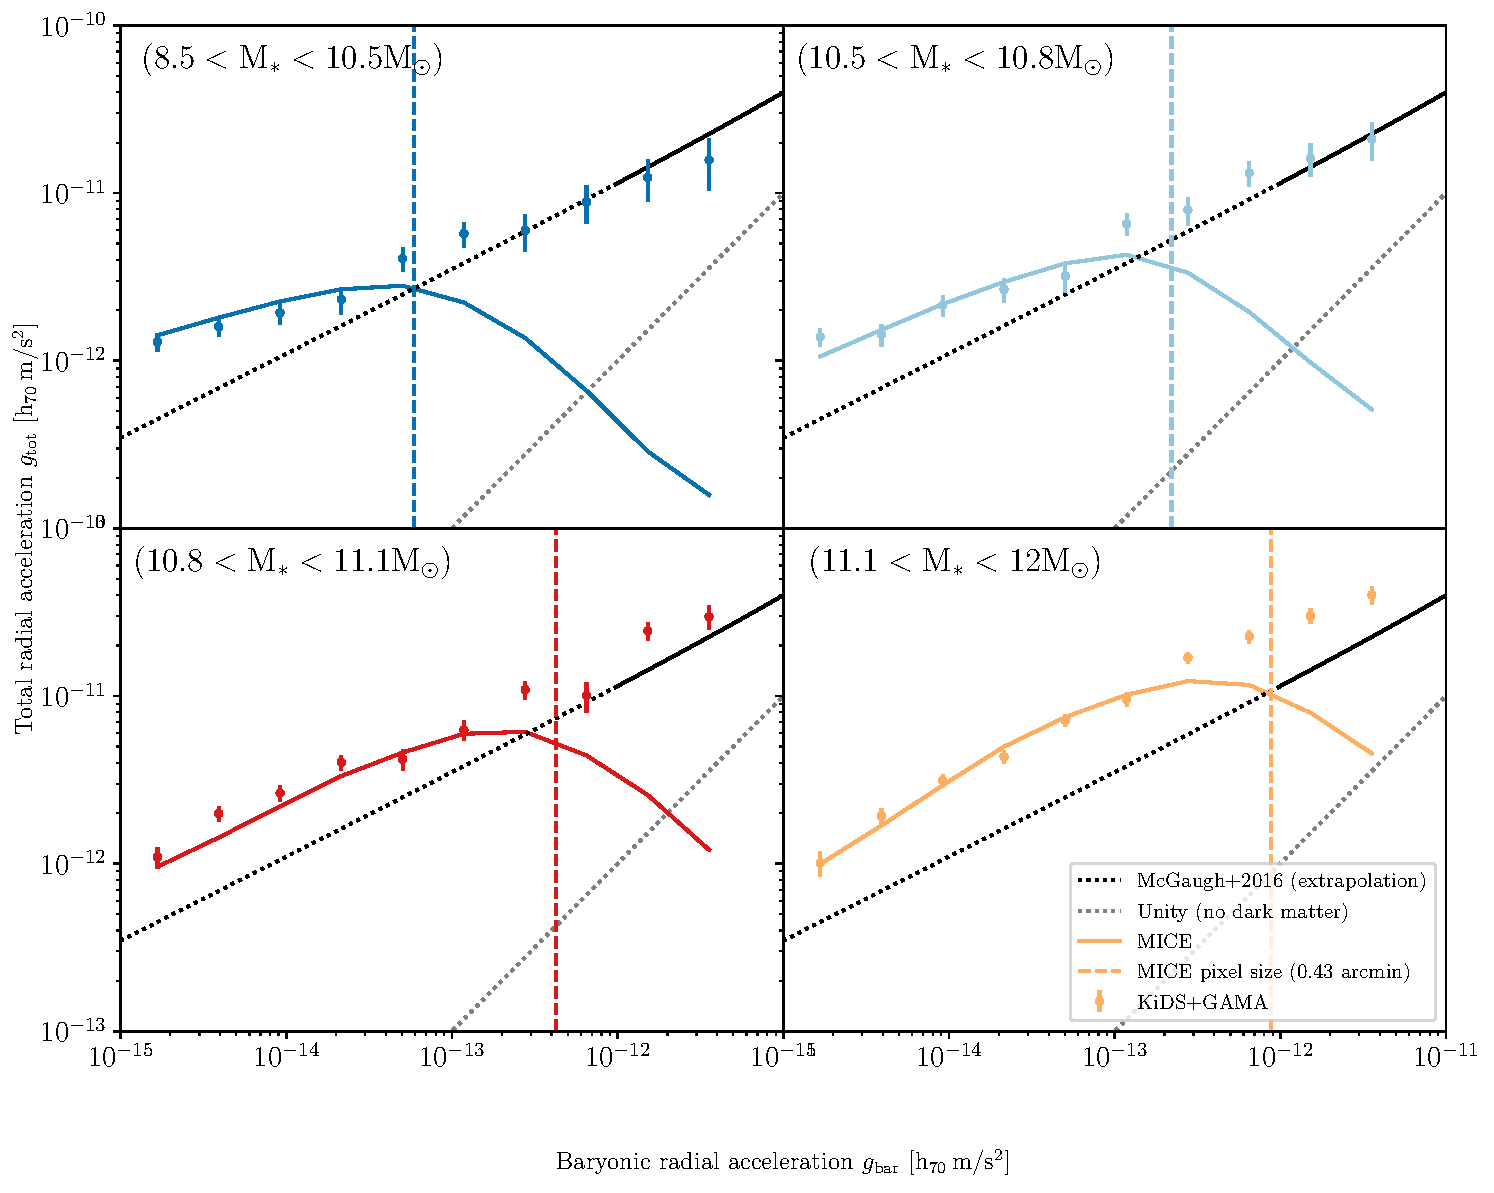
\includegraphics[width=1.0\textwidth]{Figures/RAR_GAMA+MICE_4-massbins.pdf}
	\caption{TBW}
	%\label{fig:}
\end{figure*}

\begin{figure*}
	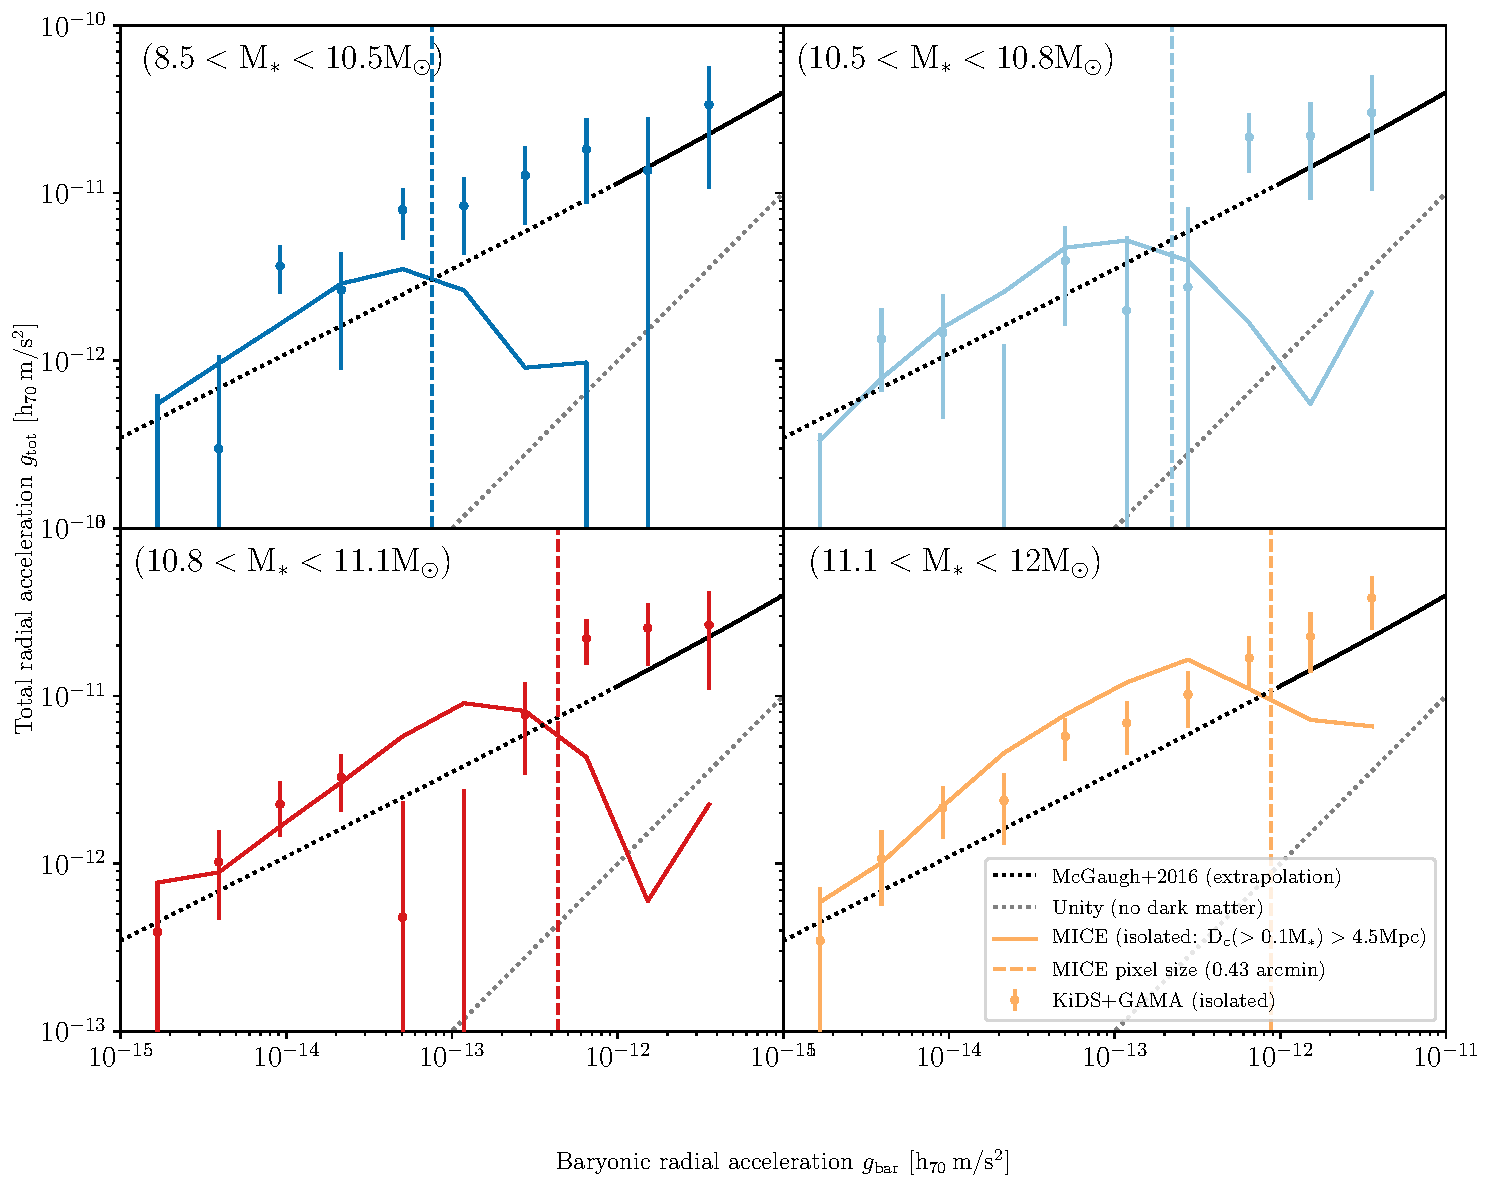
\includegraphics[width=1.0\textwidth]{Figures/RAR_GAMA+MICE_4-massbins_isolated_strong.pdf}
	\caption{TBW}
	%\label{fig:}
\end{figure*}

\begin{figure*}
	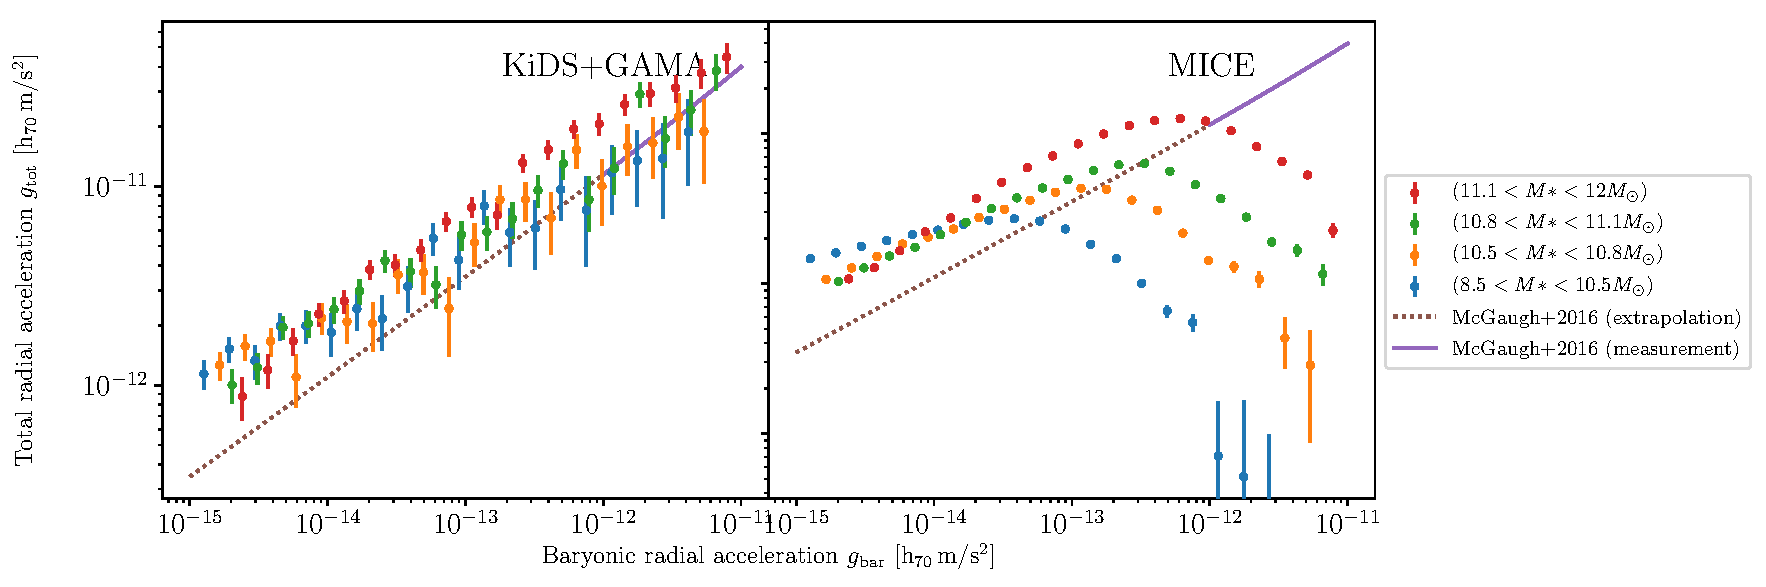
\includegraphics[width=1.0\textwidth]{Figures/RAR_KiDS+MICE_massbins-8p5_10p5_10p8_11p1_12p0_transverse.pdf}
	\caption{TBW}
	%\label{fig:}
\end{figure*}


\section{Discussion and conclusion}
\label{sec:discon}
Write at the end.

\section*{Acknowledgements}
Write at the end.

\begin{comment}
V. Demchenko acknowledges the Higgs Centre Nimmo Scholarship and the Edinburgh Global Research Scholarship. J. Harnois-D{\'e}raps is supported by the European Commission under a Marie-Sk{\l}odowska-Curie European Fellowship (EU project 656869). M. Bilicki is supported by the Netherlands Organization for Scientific Research, NWO, through grant number 614.001.451. C. Heymans acknowledges support from the European Research Council under grant number 647112. H. Hoekstra acknowledges support from Vici grant 639.043.512, financed by the Netherlands Organization for Scientific Research. K. Kuijken acknowledges support by the Alexander von Humboldt Foundation. H. Hildebrandt is supported by an Emmy Noether grant (No. Hi 1495/2-1) of the Deutsche Forschungsgemeinschaft. P. Schneider is supported by the Deutsche Forschungsgemeinschaft in the framework of the TR33 `The Dark Universe'. E. van Uitert acknowledges support from an STFC Ernest Rutherford Research Grant, grant reference ST/L00285X/1.

Computations for the $N$-body simulations were performed in part on the Orcinus supercomputer at the WestGrid HPC consortium (\url{www.westgrid.ca}), in part on the GPC supercomputer at the SciNet HPC Consortium. SciNet is funded by: the Canada Foundation for Innovation under the auspices of Compute Canada; the Government of Ontario; Ontario Research Fund - Research Excellence; and the University of Toronto.

This research is based on data products from observations made with ESO Telescopes at the La Silla Paranal Observatory under programme IDs 177.A-3016, 177.A-3017 and 177.A-3018, and on data products produced by Target OmegaCEN, INAF-OACN, INAF-OAPD and the KiDS production team,  on behalf of the KiDS consortium. OmegaCEN and the KiDS production team acknowledge support by NOVA and NWO-M grants. Members of INAF-OAPD and INAF-OACN also acknowledge the support from the Department of Physics \& Astronomy of the University of Padova, and of the Department of Physics of Univ. Federico II (Naples).

GAMA is a joint European-Australasian project based around a spectroscopic campaign using the Anglo-Australian Telescope. The GAMA input catalogue is based on data taken from the Sloan Digital Sky Survey and the UKIRT Infrared Deep Sky Survey. Complementary imaging of the GAMA regions is being obtained by a number of independent survey programs including GALEX MIS, VST KiDS, VISTA VIKING, WISE, Herschel-ATLAS, GMRT and ASKAP providing UV to radio coverage. GAMA is funded by the STFC (UK), the ARC (Australia), the AAO, and the participating institutions. The GAMA website is \url{www.gama-survey.org}.

This work has made use of CosmoHub \cite[]{carretero2017}. CosmoHub has been developed by the Port d'Informaci{\'o}n Cient{\'i}fica (PIC), maintained through a collaboration of the Institut de F{\'i}sica d'Altes Energies (IFAE) and the Centro de Investigaciones Energ{\'e}ticas, Medioambientales y Tecnol{\'o}gicas (CIEMAT), and was partially funded by the ``Plan Estatal de Investigaci{\'o}n Cient{\'i}fica y T{\'e}cnica y de Innovaci{\'o}n'' program of the Spanish government.

This work has made use of {\scshape python} (\url{www.python.org}), including the packages {\scshape numpy} (\url{www.numpy.org}) and {\scshape scipy} (\url{www.scipy.org}). Plots have been produced with {\scshape matplotlib} \cite[]{hunter2007matplotlib}. The mock shear profiles from MICE are computed using {\scshape TreeCorr} (\url{https://pypi.python.org/pypi/TreeCorr}).

\emph{Author contributions:} All authors contributed to the development and writing of this paper. The authorship list is given in three groups: the lead authors (M. Brouwer, V. Demchenko, J. Harnois-D{\'e}raps), followed by two alphabetical groups. The first alphabetical group includes those who are key contributors to both the scientific analysis and the data products. The second group covers those who have either made a significant contribution to the data products, or to the scientific analysis.
end{comment}
\end{comment}
%%%%%%%%%%%%%%%%%%%%%%%%%%%%%%%%%%%%%%%%%%%%%%%%%%

%%%%%%%%%%%%%%%%%%%% REFERENCES %%%%%%%%%%%%%%%%%%

% The best way to enter references is to use BibTeX:

\bibliographystyle{mnras}
\bibliography{biblio}


%%%%%%%%%%%%%%%%%%%%%%%%%%%%%%%%%%%%%%%%%%%%%%%%%%

%%%%%%%%%%%%%%%%%%%%%%%%%%%%%%%%%%%%%%%%%%%%%%%%%%


% Don't change these lines
\bsp	% typesetting comment
\label{lastpage}
\end{document}

% End of mnras_template.tex
